\documentclass[11pt]{article}
\usepackage[utf8]{inputenc}
\usepackage{graphicx}
\graphicspath{ {images/} }
\usepackage{amsmath}

\title{Coursework 1 – Transient Conduction}
\author{Adam Duncan}
\date{\today}

\begin{document}

\maketitle

\section{\emph{Part A: Using lumped capacitance}}
\subsection{Assumptions}
\begin{itemize}
	\item Internal temperature of the steel ball is uniform at any time t.
	\item No change in water temperature
	\item No heat transfer by radiation
	\item Material is standard carbon steel
	\item Material properties constant (taken at average temperature $T = 469 ^{o}C$)
\end{itemize}
\subsection{Schematic}
\begin{figure}[h]
	\centering
	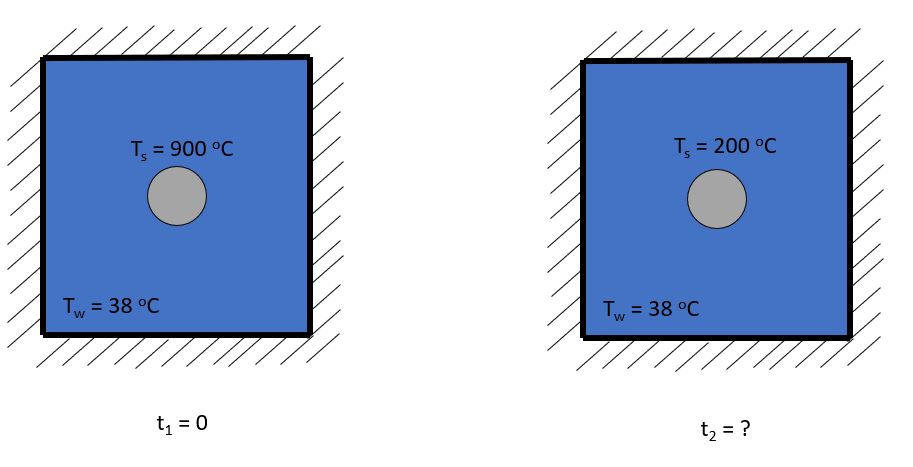
\includegraphics[width=0.85\textwidth]{part_a_fig}
	\caption{Part A schematic at initial and final state.}
	\label{fig:schem_a}
\end{figure}
\subsection{Analysis}
Energy balance for closed system gives the following equation.
\begin{equation}
	Bi = \frac{h L_{c}}{k}
\end{equation}
Where $h$ is conductivity [W/mK]
\begin{equation}
	t=\frac{f_{0} \rho C_{p} R^{2}}{k}
\end{equation}
\section{\emph{Part B: Lumped capacitance justification}}

\section{\emph{Part C: Transient conduction}}

\section{\emph{Part D: Non-infinite water bath}}

\section{\emph{Part E: Equilibrium temperature}}
\end{document}
